\documentclass{beamer}
\usetheme{default}
\usepackage{amsmath, amssymb}
\usepackage{graphicx}
\usepackage{multirow}
\usepackage{subcaption}

\title{Forward-Mode Automatic Differentiation}
\subtitle{CMSC22300 Final Project}
\author{Jay Shen}
\date{}

\begin{document}

\begin{frame}
\titlepage
\end{frame}

\begin{frame}{What is Automatic Differentiation?}
\begin{itemize}
  \item \textbf{Symbolic}: manipulates expressions $\Rightarrow$ expression swell
  \item \textbf{Numerical}: finite differences $\Rightarrow$ approximation error
  \item \textbf{Automatic}: exact derivatives via operator overloading
\end{itemize}
\vspace{1em}
This project implements forward-mode AD in Haskell using \textbf{dual numbers}.
\end{frame}

\begin{frame}[fragile]{Dual Numbers}
A dual number carries a value and its derivative:
\begin{verbatim}
data Dual a = Dual { primal :: a, tangent :: a }
\end{verbatim}
\vspace{0.5em}
Arithmetic encodes differentiation rules, e.g.\ the product rule:
\[
(x, x') \cdot (y, y') = (xy,\; x'y + xy')
\]
\vspace{0.5em}
\texttt{Num}, \texttt{Fractional}, and \texttt{Floating} instances encode the chain rule for all elementary operations.
\end{frame}

\begin{frame}[fragile]{Differentiation Combinators}
\begin{verbatim}
var x      = Dual x 1
diff f     = \x -> tangent (f (var x))
grad f xs  = [partial derivatives]
\end{verbatim}
\vspace{0.5em}
\texttt{diff} returns a first-class function, so higher-order derivatives come from composition:
\begin{itemize}
  \item \texttt{diff f} $= f'$
  \item \texttt{(diff . diff) f} $= f''$
  \item \texttt{(diff . diff . diff) f} $= f'''$
\end{itemize}
\end{frame}

\begin{frame}{Linear Regression}
Minimize MSE over $n=50$ noisy samples from $y = mx + b$:
\[
L(m, b) = \frac{1}{n} \sum_{i=1}^{n} (y_i - (mx_i + b))^2
\]
Gradient descent with $\eta = 0.001$, 1000 steps:
\vspace{0.5em}
\begin{center}
\begin{tabular}{lccc}
\hline
\textbf{Param} & \textbf{True} & \textbf{Fitted} & \textbf{Loss} \\
\hline
$m$ & 3.0 & 3.029 & \multirow{2}{*}{0.212} \\
$b$ & 1.0 & 0.874 & \\
\hline
\end{tabular}
\end{center}
\end{frame}

\begin{frame}{Logistic Regression}
Binary classification with cross-entropy loss:
\[
L(w, b) = -\frac{1}{n} \sum_{i=1}^{n} \bigl[ y_i \log p_i + (1-y_i)\log(1-p_i) \bigr]
\]
Gradient descent with $\eta = 0.1$, 1000 steps:
\vspace{0.5em}
\begin{center}
\begin{tabular}{lccc}
\hline
\textbf{Param} & \textbf{Fitted} & \textbf{Loss} & \textbf{Accuracy} \\
\hline
$w$ & 3.360 & \multirow{2}{*}{0.032} & \multirow{2}{*}{99\%} \\
$b$ & 0.106 & & \\
\hline
\end{tabular}
\end{center}
\end{frame}

\begin{frame}{Higher-Order Derivatives}
\begin{figure}
  \centering
  \begin{subfigure}[b]{0.48\textwidth}
    \centering
    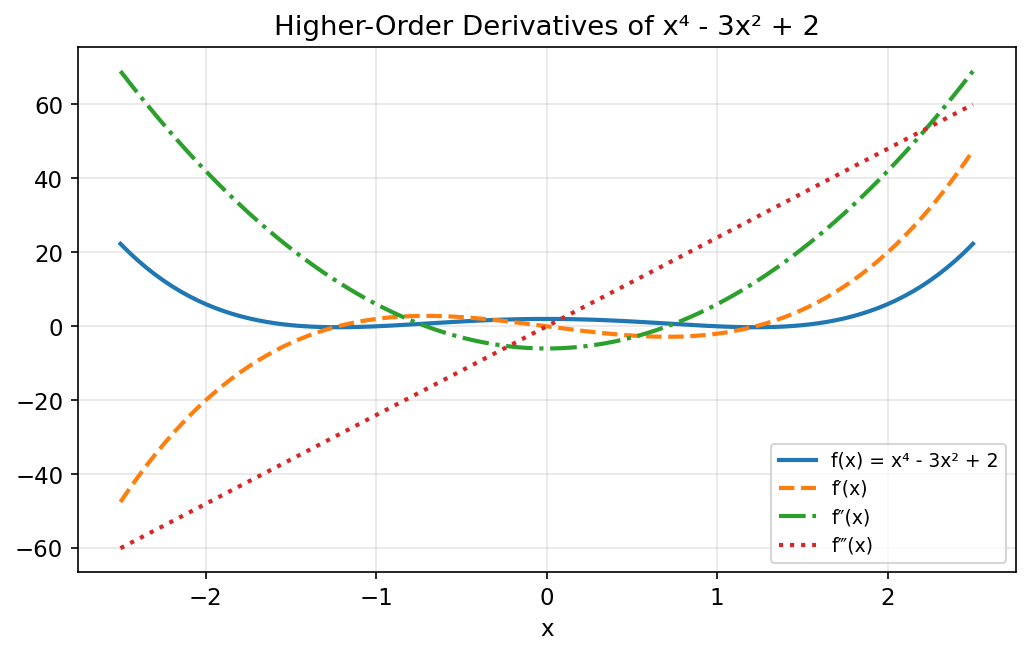
\includegraphics[width=\textwidth]{../visualization/images/polynomial.png}
    \caption{$x^4 - 3x^2 + 2$}
  \end{subfigure}
  \hfill
  \begin{subfigure}[b]{0.48\textwidth}
    \centering
    \includegraphics[width=\textwidth]{../visualization/images/sinusoidal.png}
    \caption{$\sin(x)$}
  \end{subfigure}
  \\[0.5em]
  \begin{subfigure}[b]{0.48\textwidth}
    \centering
    \includegraphics[width=\textwidth]{../visualization/images/exponential.png}
    \caption{$e^x$}
  \end{subfigure}
  \hfill
  \begin{subfigure}[b]{0.48\textwidth}
    \centering
    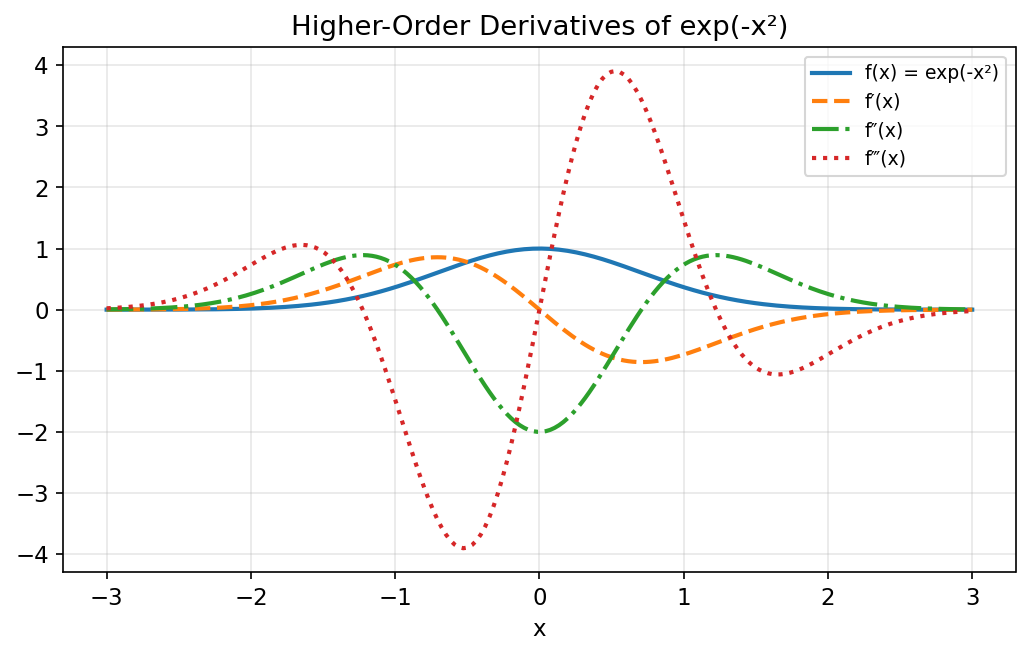
\includegraphics[width=\textwidth]{../visualization/images/composite.png}
    \caption{$e^{-x^2}$}
  \end{subfigure}
\end{figure}
\end{frame}

\begin{frame}{Gradient Field}
$f(x,y) = \sin(x)\cos(y)$ over $[-\pi, \pi]^2$:
\begin{figure}
  \centering
  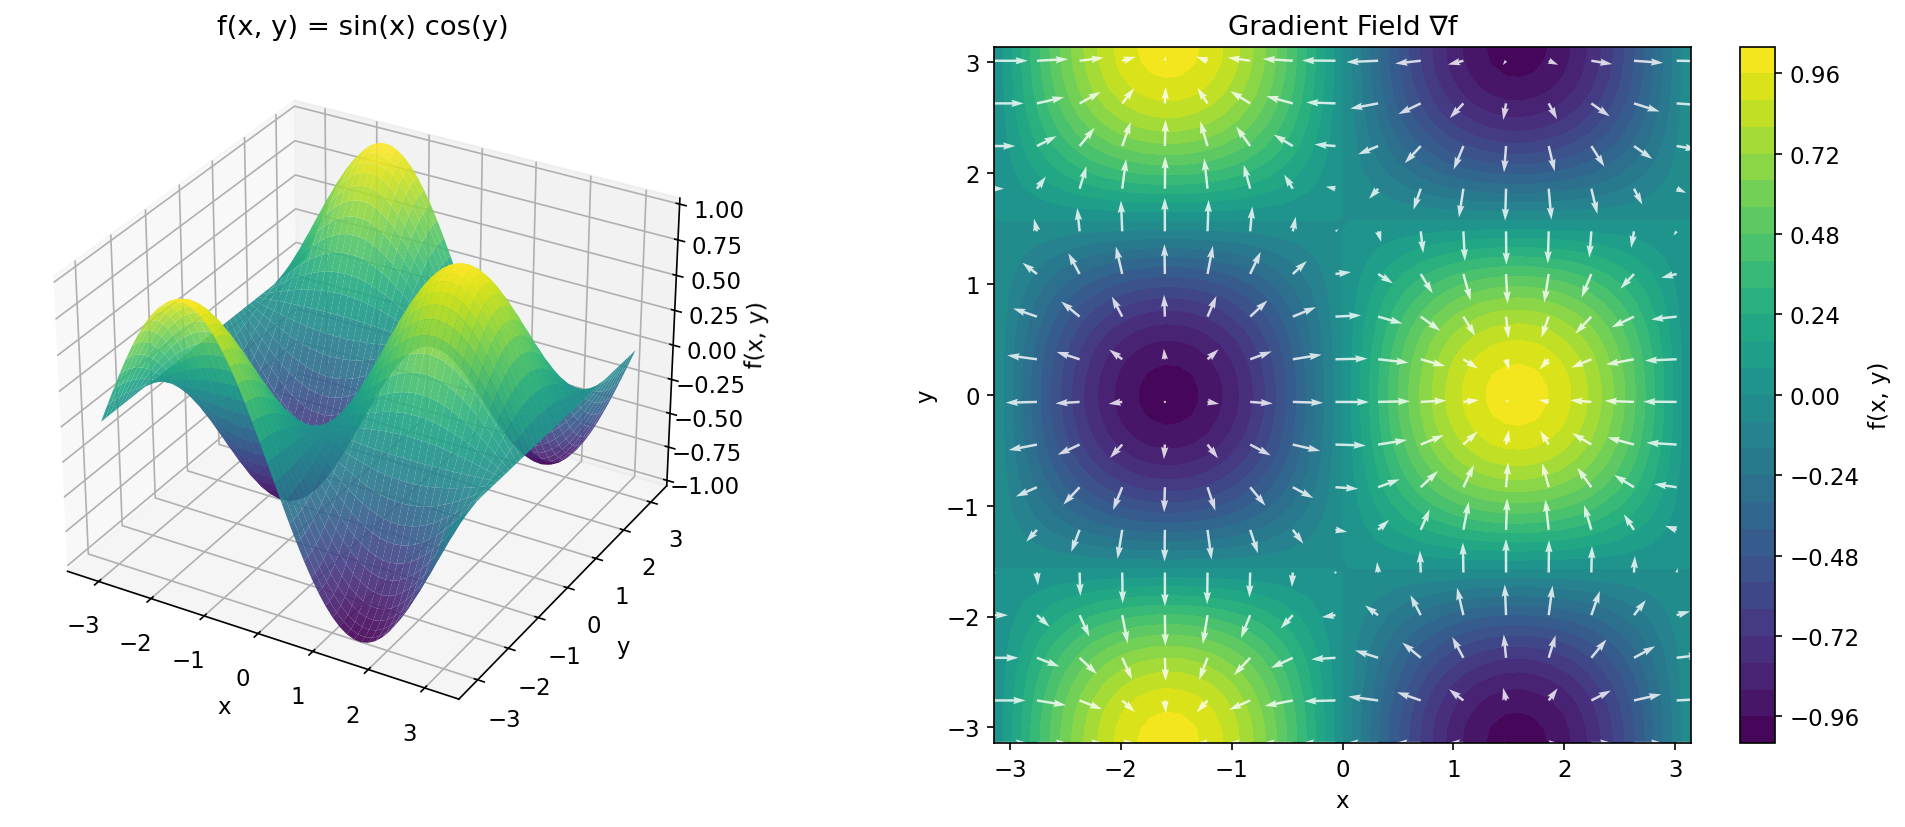
\includegraphics[width=0.85\textwidth]{../visualization/images/gradient_field.png}
\end{figure}
\end{frame}

\begin{frame}{Summary}
\begin{itemize}
  \item Forward-mode AD via dual numbers gives exact derivatives
  \item Haskell's typeclass system makes the implementation concise
  \item Higher-order derivatives via simple function composition
  \item Gradients accurate enough to drive gradient descent to convergence
\end{itemize}
\end{frame}

\end{document}
